%% -*- coding: utf-8 -*-
\documentclass[12pt,pagesize,paper=192mm:108mm,landscape]{scrbook} 
%1920x1080 1280x720
\areaset[current]{192mm}{108mm}
\usepackage{calc}
\usepackage[T2A]{fontenc}
\usepackage[utf8]{inputenc}
\usepackage[english,russian]{babel}
\usepackage{microtype}
\usepackage{misccorr}
\usepackage{cmap}
%\usepackage[unicode=true]{hyperref}
\usepackage{graphicx}
\usepackage{amssymb}
\usepackage{amsmath}
%\usepackage{srcltx}
\usepackage{textcomp}
\usepackage{xspace}
%научные символы и смайлики \smiley \frownie
\usepackage{wasysym}
\usepackage{ccicons}
\begin{document}
\begin{titlepage}
  \vspace*{-0.5em}
  \begin{center}    
    % \hspace*{3em}
    % \begin{minipage}[t]{3em}
    %   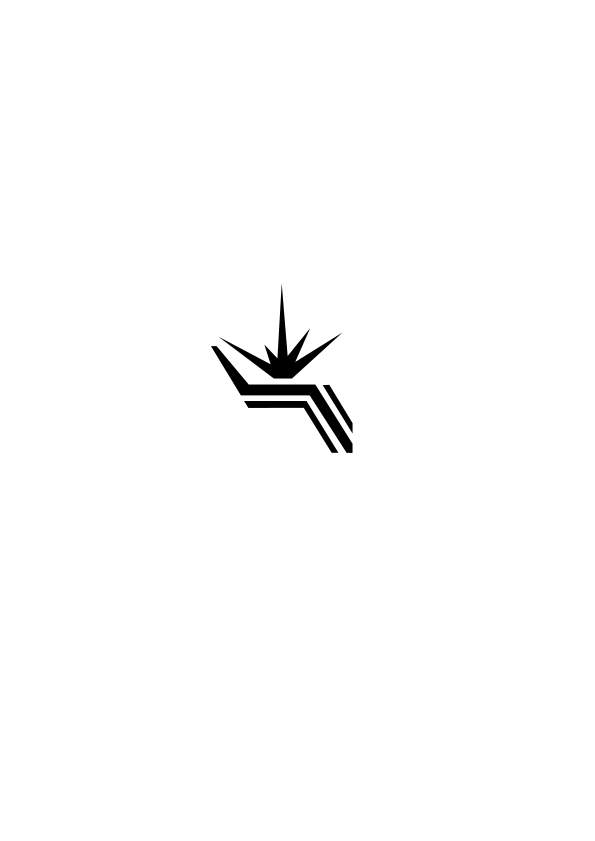
\includegraphics[width=\textwidth]{../BINP-logo}
    % \end{minipage}\hfill
    % \begin{minipage}{0.23\linewidth}
    % 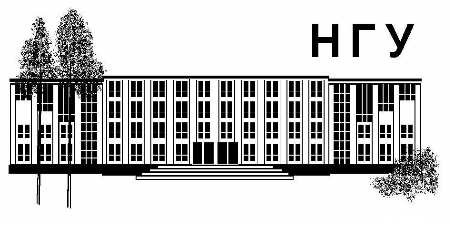
\includegraphics[width=\textwidth]{../NSU-logo}
    % \end{minipage}
    % \hfill
    % \hspace*{6em}

    
    % Кафедра теоретической физики физического факультета НГУ
    % \medskip

    % \Large
    % Профессор Грабовский А.\,В.
    % \smallskip

    % \huge
    % \textbf{Общая теория относительности}
    % \smallskip

    % \Large
    % Лекция № 10
     \vfill

     \normalsize
     \begin{minipage}{0.95\linewidth}
       Единицы измерения больших расстояний: астрономическая единица,
       световой год, парсек. Характерные масштабы во вселенной:
       расстояние до Солнца, до ближайшей звезды, размер Млечного
       пути, количество звезд в нем, расстояние до ближайшей
       галактики, местная группа, ее размер, масса, количество
       галактик в ней, Сверхскопление Девы, его размер, кластер Девы,
       его размер, масса, количество галактик в нем, расстояние от нас
       до него, количество суперкластеров в наблюдаемой
       вселенной. Крупномасштабная структура вселенной: пустоты,
       (галактические) стены, филаменты (галактические нити), их
       характерный масштаб. Моделирование крупномасштабной структуры
       вселенной. Однородность и изотропность пространства на
       масштабах больше 300\,Мпс. Фотометрический парадокс
       Ольберса. Красное смещение $z$. Экспериментальный закон Хаббла,
       постоянная Хаббла, скорость разбегания галактик, расширение
       вселенной. Хаббловские расстояние и время. Принцип
       Коперника. Обзоры неба. Определение возраста вселенной по
       Хаббловскому времени, по относительному содержанию различных
       элементов во вселенной, по наблюдению старых звезд в гало нашей
       галактики. Критическая плотность $\rho_c$. Относительная
       плотность $\Omega=\rho/\rho_c$ определенного вида энергии в
       долях критической плотности. Оценка плотности светящейся
       материи, оценка плотности барионной материи. Кривые вращения
       галактик и определение массы галактики по теореме
       вириала. Интерпретация результатов как наличие темной материи,
       оценка массы темной материи. Горячая и холодная темная материя.
    \end{minipage}
    \vfill

    \normalsize \ccbysa\hspace{0.5em}  Новосибирск 2022
  \end{center}
\end{titlepage}
\end{document}
